% !TeX spellcheck = pt_BR
%\chapter[Semana 7]{}
\chapter[Teoria de Cauchy]{Teoria de Cauchy:\\ Integração no plano complexo}
\chaptermark{}


\hfill%
\begin{minipage}{12cm}
	\begin{flushright}
		\rightskip=0.5cm
		\textit{``At the basis of the distance concept lies, for example, 
		the concept of a convergent point sequence and their defined limits,
		and one can, choosing these ideas as those fundamental to the point 
		set theory, eliminate the notions of distance ... Thirdly, 
		we can associate with each point of the set certain parts of the space
		called neighborhoods, and these can again be made building stones of the 
		theory with the elimination of the distance concept. Here the view
		of a set is in consideration of the association between elements and
		subsets.''}
		\\[0.1cm]
		\rightskip=0.5cm
		---F. Hausdorff, 1949
	\end{flushright}
\end{minipage}



\section{A Integral Complexa}

\begin{lema}
Sejam $U \subset \C$ um domínio e $f:U \to \C$ uma função holomorfa. Se $f'(z) = 0$ para
todo ponto $z\in U$, então $f$ é uma função constante.
\end{lema}

\begin{definicao}[Integral complexa]
\label{def:integral-complexa}
\index{Integral complexa}
A integral da função $f$ ao longo do caminho $\y$ é
o número complexo
\begin{equation*}
    \int_{\y} f(z) dz = \int_a^b f(\y(t))\y'(t) dt,
\end{equation*}
sendo $\y:[a,b]\to\C$ um caminho suave e
$f:U \to \C$ função contínua com $U$ domínio.
\end{definicao}

\begin{definicao}
Sejam $f$ e $U$ como na Definição \ref{def:integral-complexa} e
$\y = \y_1*\y_2*\cdots*\y_n$ um caminho suave por partes em $U$.
A integral de $f(z)$ ao longo de $\y$ é o número complexo
\begin{equation*}
    \int_{\y} f(z)dz = \sum_{i=1}^n\int_{\y_i} f(z)dz.
\end{equation*}
\end{definicao}



\section[Primitivas e o Teorema Fundamental do Cálculo]
{Primitivas e o Teorema Fundamental\\ do Cálculo}

\begin{definicao}
\label{def:primitiva-complexa}
Seja $f:U \to \C$ uma função contínua com $U\subset\C$ domínio. Uma função $F:U\to\C$
é chamada primitiva de $f$ se $F$ é holomorfa em $U$ e $F'(z) = f(z), \forall z\in U$.
\end{definicao}

\begin{teorema}

Sejam $U\subset\C$ domínio, $f:U\to\C$ função contínua,
$F$ uma primitiva de $f$ em $U$ e $\y$ um caminho suave por partes em $U$ unindo $z_0$ a $z_1$. Então
\begin{equation*}
    \int_{\y} f(z)dz = F(z_1) - F(z_0).
\end{equation*}
Em particular, se o caminho é fechado então
\begin{equation*}
    \int_{\y} f(z)dz = 0.
\end{equation*}
\end{teorema}

\begin{proposicao}
Seja $\displaystyle{ f(z) = \sum_{n=0}^{\infty} a_n(z-z_0)^n }$
definida por uma série de potências com raio de convergência $R>0$.
Então a função
\begin{equation*}
    F(z) = \sum_{n=0}^{\infty} \frac{a_n}{n+1}(z-z_0)^{n+1}
\end{equation*}
é uma primitiva de $f$ e a série que a define converge para $|z-z_0| < R$.
\end{proposicao}

\begin{lema}[Lema Técnico]
\label{lema-tecnico}
Sejam $U\subset\C$ um domínio, $f:U\to\C$ uma função contínua e
$\y(t), a\leq t\leq b$ um caminho suave por partes em $U$, de comprimento $l(\y)$.
Seja $K\geq 0$ um número real tal que $|f(\y(t))| \leq K$ para todo $a\leq t\leq b$. Então
\begin{equation*}
    \left| \int_{\y}f(z)dz \right| \leq Kl(\y).
\end{equation*}
\end{lema}

\begin{teorema}
Seja $f:U\to \C$ uma função contínua definida no domínio $U\subset\C$. As seguintes afirmações são equivalentes:
\begin{enumerate}[(i)]
    \item $f$ tem uma primitiva em $U$
    \item $\int_{\y} f(z) dz = 0$ para qualquer caminho $\y$ fechado e suave por partes em $U$.
    \item $\int_{\lambda} f(z) dz$ só depende dos pontos inicial e final de qualquer caminho $\lambda$ suave por partes em $U$.
\end{enumerate}
\end{teorema}


\section[Os teoremas de Cauchy]{Os teoremas de Cauchy}

\begin{teorema}[Teorema de Cauchy-Goursat]
\label{teo:cauchy-goursat}
\index{Teorema!de Cauchy-Goursat}
Sejam $U$ um domínio em $\C$ e $f: U \to \C$ uma função holomorfa. Suponha que $\Delta \subset U$ é uma triângulo que limita
uma região inteiramente contida em $U$. Então
\begin{equation*}
    \int_{\Delta} f(z) dz = 0.
\end{equation*}
\end{teorema}


\begin{definicao}[Domínio estrelado]
\index{Domínio estrelado}
Seja $U\subset\C$ um domínio. Dizemos que $U$ é estrelado se existe um ponto $z_0\in U$
tal que dado qualquer ponto $z\in U$, o segmento de reta $\overline{z_0z}$ está inteiramente contido em $U$. 
O ponto $z_0$ é chamado um centro do domínio $U$.
\end{definicao}


\begin{corolario}
Sejam $U\subset\C$ um domínio estrelado e $f:U\to\C$ uma
função holomorfa. Então $f$ admite uma primitiva em $U$.
\end{corolario}


\begin{corolario}[Teorema de Cauchy-Goursat bis]
Sejam $U\subset\C$ um domínio estrelado e $f:U\to\C$ uma função holomorfa.
Se $\y$ é um caminho fechado suave por partes em $U$, então
\begin{equation*}
    \int_{\y} f(z) dz = 0.
\end{equation*}
\end{corolario}


\begin{teorema}[Fórmula Integral de Cauchy]
\label{teo:form-integral-cauchy}
\index{Fórmula!Integral de Cauchy}
Seja $f:U \to \C$ uma função holomorfa definida no domínio $U\subset\C$.
Sejam $\overline{D}(z_0, r_0)$ um disco fechado inteiramente contido em $U$ e $\y$ sua fronteira, orientada compativelmente. 
Se $z$ é um ponto qualquer no interior de $\overline{D}(z_0, r_0)$ então
\begin{equation*}
    f(z) = \frac{1}{2\pi i}\int_{\y} \frac{f(w)}{w-z}dw.
\end{equation*}
\end{teorema}


\begin{corolario}
Seja $f:U\to\C$ holomorfa com $U$ domínio. Então $f$ tem derivadas de todas as ordens em todos os pontos de $U$ e
\begin{equation*}
    f^{(n)}(z) = \frac{n!}{2\pi i}\int_{\y} \frac{f(w)}{(w-z)^{n+1}}dw, \forall z\in U,
\end{equation*}
onde $\y$ é qualquer circunferência centrada em $z$, percorrida no sentido anti-horário e limitando um disco fechado contido em $U$.
\end{corolario}


\begin{corolario}[Estimativas de Cauchy]
\label{cor-estimativas-cauchy}
\index{Estimativas de Cauchy}
Seja $f$ uma função holomorfa definida no disco $D(z_0, R)$ e suponha que
$|f|\leq K$ em $D(z_0, R)$. Então
\begin{equation*}
    |f^{(n)}(z_0)| \leq \frac{n!K}{R^n}.
\end{equation*}
\end{corolario}


\begin{corolario}[Teorema de Liouville]
\label{teo-liouville}
\index{Teorema!de Liouville}
Seja $f$ função inteira. Se existe $K\geq 0$ tal que $|f(z)|\leq K$ então $f$ é uma função constante.
\end{corolario}


\begin{lema}
Seja $D(a,r), r>0$, um disco e $f: D(a,r)\to\C$ uma função holomorfa. 
Se a imagem de $f$ está contida no interior de uma circunferência $|w| - \alpha$, então $f$ é uma função constante.
\end{lema}


\begin{corolario}[Princípio do Módulo Máximo]
\label{principio-modulo-maximo}
\index{Princípio do Módulo Máximo}
\index{Teorema!do Módulo Máximo}
Sejam $U$ um domínio em $\C$ e $f:U\to\C$ uma função holomorfa.
Suponha que existe um ponto $a\in U$ tal que $|f(a)| \geq |f(z)|, \forall z\in U$. Então $f$ é uma função constante.
\end{corolario}


\begin{teorema}
Sejam $f:U\to\C$ uma função holomorfa com $U$ domínio e $z_0\in U$ qualquer.
Então
\begin{equation*}
    f(z) = \sum_{n=0}^{\infty} \frac{f^{(n)}(z_0)}{n!}(z-z_0)^n,
\end{equation*}
ou seja, $f$ é dada por sua série de Taylor de centro em $z_0$ e, portanto, é uma função analítica.
Ademais, essa série converge em qualquer disco (aberto) $D(z_0, r) \subset U$, isto é, o raio de convergência $R$ da série acima é a menor entre as distâncias de $z_0$ aos pontos da fronteira de $U$.
\end{teorema}


\begin{teorema}[Teorema de Cauchy]
\label{teo-cauchy}
\index{Teorema!de Cauchy}
Sejam $U\subset\C$ um domínio e $f:U\to\C$ uma função holomorfa. Seja $V\subset U$ um subconjunto fechado e limitado, cuja fronteira $\partial V$ consiste de um número finito de curvas de Jordan
suaves por partes, $\partial V = \y_1\cup\cdots\y_n$, e tal que
$V\setminus\partial V$ é domínio. Então
\begin{equation*}
    \int_{\partial V} f(z) dz = 0.
\end{equation*}
\end{teorema}

\begin{teorema}[Fórmula Integral de Cauchy bis]
\label{form-integral-cauchy-bis}
Seja $f:U\to\C$ uma função holomorfa definida no domínio $U$. Seja $V$ uma região fechada e limitada inteiramente contida em $U$, 
cuja fronteira $\partial V$ é uma curva de Jordan suave por partes, orientada no sentido anti-horário, sendo $V\setminus\partial V$ um domínio.
Se $z_0$ é um ponto qualquer no interior de $V$, então
\begin{equation*}
    f(z_0) = \frac{1}{2\pi i}\int_{\partial V} \frac{f(w)}{w-z_0} dw.
\end{equation*}
\end{teorema}


\begin{teorema}[Teorema de Morera]
\label{teo-morera}
\index{Teorema!de Morera}
Sejam $U\subset\C$ domínio e $f:U\to\C$ uma função contínua.
Se $\int_{\Delta} f(z) dz = 0$ para todo caminho triangular $\Delta\subset U$, então $f$ é holomorfa em $U$.
\end{teorema}


\section[Singularidades, resíduos e o Teorema de Rouché]{Singularidades, resíduos e o Teorema de Rouché}

\begin{teorema}[Teorema de Laurent]
\label{teo-laurent}
\index{Teorema!de Laurent}
Seja $f$ uma função holomorfa no anel $A(a, \rho_1, \rho_2)$. Então
\begin{equation*}
    f(z) = \sum_{m=1}^{\infty} b_m\frac{1}{(z-a)^m} + \sum_{n=0}^{\infty} a_n(z-a)^n,
\end{equation*}
sendo que a primeira série converge absolutamente fora do disco fechado $\overline{D}(a, \rho_1)$
e a segunda série converge absolutamente no disco (aberto) $D(a, \rho_2)$. 
Ademais, essa expansão é única e os coeficientes $b_m$ e $a_n$ são dados por
\begin{align*}
    b_m &= \frac{1}{2\pi i}\int_{\y} f(z)(z-a)^{m-1} dz, m\geq 1 \\
    a_n &= \frac{1}{2\pi i}\int_{\y} \frac{f(w)}{(w-a)^{n+1}} dw, n\geq 0,
\end{align*}
sendo $\y$ uma circunferência de centro $a$ orientada no sentido anti-horário 
e contida no anel $A(a, \rho_1, \rho_2)$.
\end{teorema}


\begin{definicao}[Singularidades e polos]
\index{Singularidade Removível}
\index{Polos}
\index{Singularidade Essencial}
Dizemos que 
\begin{itemize}
    \item $a$ é singularidade removível de $f$ se $b_m = 0$ para $m\geq 1$;
    \item $a$ é polo de ordem $k$ de $f$ se $b_k\neq 0$ e $b_m = 0$ para $m>k$;
    \item $a$ é singularidade essencial de $f$ se $b_m\neq 0$ para infinitos valores de $m$.
\end{itemize}
\end{definicao}


\begin{proposicao}
Seja $f$ uma função holomorfa no anel $A(a, 0, \rho)$. As seguintes afirmações são equivalentes.
\begin{enumerate}[(i)]
    \item $a$ é singularidade removível de $f$;
    \item existe $\displaystyle{\lim_{z\to a} f(z)}$;
    \item $|f|$ é limitado em algum anel $A(a, 0, \delta) \subset A(a, 0, \rho)$.
\end{enumerate}
\end{proposicao}


\begin{corolario}
Se $b_m\neq 0$ para algum $m\geq 1$, então $|f|$ é ilimitado em qualquer disco de centro $a$.
\end{corolario}


\begin{proposicao}
Se $f$ é função holomorfa no anel $A(a, 0, \rho)$, então $a$ é um polo de ordem $k$ de $f$
se, e somente se, $\displaystyle{ \lim_{z\to a} (z-a)^k f(z) }$ existe e é um número complexo não nulo.
\end{proposicao}

\clearpage
\begin{corolario}
Se $f$ é holomorfa no anel $A(a, 0, \rho)$ e $a$ é polo de ordem $k$ de $f$ então
$\displaystyle{ \lim_{z\to a} |f(z)| = \infty }$.
\end{corolario}


\begin{teorema}[Teorema de Casorati-Weierstrass]
\label{teo-casorati-weierstrass}
\index{Teorema!de Casorati-Weierstrass}
Seja $f$ uma função holomorfa no anel $A(a,0,\rho)$ e suponha que $a$ é singularidade essencial de $f$.
Então, dados $0<r\leq\rho, \varepsilon > 0$ e $\alpha\in\C$, existe um número complexo $\beta$
no anel $A(a,0,r)$ tal que $|f(\beta) - \alpha| < \varepsilon$.
\end{teorema}


\begin{definicao}[Resíduo]
\label{def-residuo}
\index{Resíduo}
Se $f$ é uma função holomorfa no anel $A(a, 0, \rho)$, o resíduo de $f$ em $a$ é o coeficiente $b_1$
do termo $(z-a)^{-1}$ de sua série de Laurent com centro em $a$, denotado por $\res(f, a)$.
\end{definicao}


\begin{teorema}[Teorema dos Resíduos]
\label{teo-residuos}
\index{Teorema!dos Resíduos}
Seja $f$ uma função holomorfa num domínio $U\setminus\{ a_1, a_2, \dots, a_m \}$. Suponha que 
$\y \subset U\setminus\{ a_1, a_2, \dots, a_m \}$ é uma curva de Jordan suave por partes,
orientada no sentido anti-horário, tal que a região fechada e limitada por ela determinada está
contida em $U$ e contém todos os pontos $ a_1, a_2, \dots, a_m$. Então
\begin{equation*}
    \frac{1}{2\pi i}\int_{\y} f(z) dz = \sum_{i=1}^m \res(f, a_i).
\end{equation*}
\end{teorema}


\begin{proposicao}
Seja $f$ uma função holomorfa no anel $A(a, 0, \rho)$ e suponha que $a$ é polo de ordem 1 de $f$.
Então $\res(f,a) = \displaystyle{ \lim_{z\to a} (z-a) f(z) }$.
\end{proposicao}


\begin{proposicao}
Seja $f$ uma função holomorfa no anel $A(a, 0, \rho)$ e suponha que $a$ é polo de ordem $k>1$ de $f$.
Considere a função $g(z) = (z-a)^k f(z)$. Então
\begin{equation*}
    \res(f, a) = \frac{g^{(k-1)}(a)}{(k-1)!}.
\end{equation*}
\end{proposicao}


\begin{teorema}
\label{teo-contador-zeros}
Seja $f$ uma função holomorfa num domínio $U\setminus\{ a_1, a_2, \dots, a_m \}$. Suponha que 
$\y \subset U\setminus\{ a_1, a_2, \dots, a_m \}$ é uma curva de Jordan suave por partes,
orientada no sentido anti-horário, tal que a região fechada e limitada por ela determinada está
contida em $U$ e contém todos os pontos $ a_1, a_2, \dots, a_m$. Ademais, suponha que todos esses
pontos sejam polos de $f$ e que $f$ não tem zeros ao longo de $\y$. Então
\begin{equation*}
    \frac{1}{2\pi i}\int_{\y} \frac{f'(z)}{f(z)} dz = \mathcal{Z} - \mathcal{P},
\end{equation*}
sendo $\mathcal{Z}$ o número de zeros de $f$ na região interior a $\y$ (contados com multiplicidade)
e $\mathcal{P}$ o número de polos de $f$ na região interior a $\y$ (contados com multiplicidade).
\end{teorema}


\begin{corolario}
Nas mesmas hipóteses do Teorema \ref{teo-contador-zeros}, se $f$ e $h$ são funções holomorfas em $U$,
então
\begin{equation*}
    \frac{1}{2\pi i}\int_{\y} h(z)\frac{f'(z)}{f(z)} dz = \sum_{\xi_j} h(\xi_j)m_{\xi_j}(f),
\end{equation*}
sendo $\xi_1, \xi_2, \dots, \xi_l$ os zeros de $f$ na região interior a $\y$ e $m_{\xi_j}(f)$
a multiplicidade de $\xi_j$ como zero de $f$.
\end{corolario}


\begin{teorema}[Teorema de Rouché]
\label{teo-rouche}
\index{Teorema!de Rouché}
Sejam $f$ e $g$ duas funções holomorfas definidas num domínio $U\subset\C$. Seja $V\subset U$
uma região fechada e limitada cuja fronteira $\partial V$ é uma curva de Jordan suave por partes, com
$V\setminus\partial V$ um domínio. Se
\begin{equation*}
    |f(z) - g(z)| < |f(z)|, \forall z\in\partial V,
\end{equation*}
então $f$ e $g$ têm o mesmo número de zeros no interior de $V$, cada um deles contados com multiplicidade.
\end{teorema}

Interpretação dinâmica do resíduo?
Cálculo de integrais usando resíduos?
%
\begin{lema}
\label{lema-zeros-vezes-polos}
Se $f:U\subseteq\C\to\C$ é uma função holomorfa tendo $z_0$ como um zero de multiplicidade
$m$ e $g:U\subseteq\C\to\C$ é uma função meromorfa tendo $z_0$ como um polo de ordem $m$, então
$h(z) \equiv f(z)g(z)$ é holomorfa.
\end{lema}
%
\begin{proof}
Podemos escrever $f$ como
%
\[
f(z) = (z - z_0)^m \widetilde{f}(z),
\]
%
com $\widetilde{f}(z_0) \neq 0$, e podemos expandir $g$ em série de Laurent da seguinte
forma
%
\[
g(z) = \sum_{j=1}^m \frac{b_j}{(z - z_0)^j} + \sum_{n=1}^{\infty} a_n (z - z_0)^n.
\]
%
Daí, temos
%
\begin{align*}
    f(z)g(z) = \widetilde{f}(z)
    \left[ \sum_{j=1}^m b_j (z - z_0)^{m-j} + \sum_{n=1}^{\infty} a_n (z - z_0)^{m+n} \right].
\end{align*}
%
Como $\widetilde{f}$ e ambos os somatórios são holomorfos, segue que $h(z) \equiv f(z) \cdot g(z)$ é 
holomorfa.
\end{proof}
%
\begin{teorema}
Seja $\Omega\subseteq\C$ um domínio e $I = \dis{\bigcup_{n\in\N} I_n} \subseteq\R$ onde,
para cada $n\in\N$, $I_n$ é um intervalo fechado em $\R$ e $\sharp I_n \cap I_m = 0, 1$ se
$n\neq m$. Suponha, ainda, que
%
\begin{itemize}
    \item para cada $x\in I\subseteq\R$ a aplicação 
    $z\longmapsto f(z,x)$ é holomorfa;
    \item $(z,x) \longmapsto f(z,x)$ é contínua;
    \item para qualquer compacto $K\subseteq U$ temos
    %
    \[
    \int_I\, \sup_{z\in K} |f(z,x)| \, dx < +\infty.
    \]
    %
    Então
    %
    \[
    z \longmapsto \int_I f(z,x) \, dx \equiv g(z)
    \]
    %
    é holomorfa em $\Omega$.
\end{itemize}
%
\end{teorema}
%
Aqui fazemos uma observação acerca da notação. Se temos
%
\[
I = \bigcup_{n=1}^{\infty} I_n, \qquad I_n = [a_n, b_n],
\]
%
então para qualquer função integrável $g:\R\to\R$ escrevemos
%
\[
\int_I g(x) \, dx 
\equiv \sum_{n=1}^{\infty} \int_{I_n} g(x) \, dx 
\equiv \sum_{n=1}^{\infty} \int_{a_n}^{b_n} g(x) \, dx.
\]
%
\begin{definicao}[Continuidade uniforme]
\label{def-cont-unif}
\index{Função!uniformemente contínua}
Uma função $f:U\subseteq\C\to\C$ é uniformemente contínua em $U$ se dado $\e > 0$
existe $\delta > 0$ tal que para quaisquer $z,w$ tais que $|z-w| < \delta$ então
$|f(z) - f(w)| < \e$.
\end{definicao}
%
\begin{figure}[H]\centering
    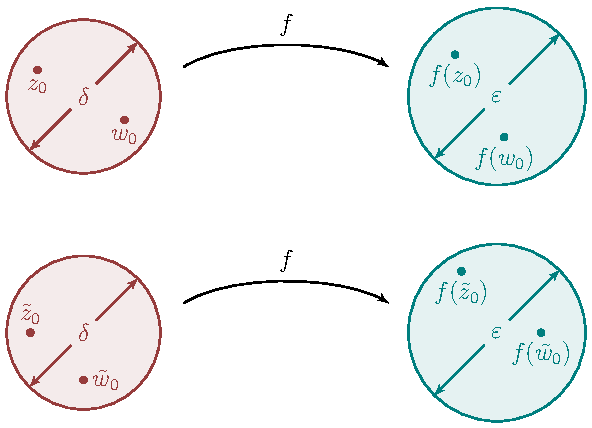
\includegraphics{Figuras/continuidade uniforme.pdf}
\end{figure}
%
\begin{teorema}
Seja $f:U\subseteq\R^n\to\C$ uma função contínua. Se $K\subseteq U$ é um compacto,
então $f\big|_K$ é uniformemente contínua.
\end{teorema}
%
\begin{figure}[H]\centering
    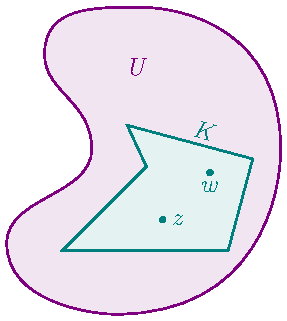
\includegraphics{Figuras/K em U.pdf}
\end{figure}
%
\begin{proof}
Suponha que $f\big|_K$ não é uniformemente contínua. Então, dado $\e>0$, para
cada $n\in\N$ e $\delta_n = 1/n$ podemos encontrar $z_n, w_n\in K$ tais que
$\|z_n - w_n\| < \delta_n$ mas $\e\leq |f(z_n) - f(w_n)|$.
%
\begin{figure}[H]\centering
    \includegraphics{Figuras/f|K não uniforme.pdf}
\end{figure}
%
Como $K$ é compacto, existe uma subsequência $(z_{n_k})\subset (z_n)$ tal que
$z_{n_k} \to z\in K$. Considere a sequência $(w_{n_k})$. Pelo mesmo argumento, existe
uma subsequência $(w_{n_{k_p}})\subset (w_{n_k})$ tal que
$w_{n_{k_p}} \to w\in K$. É claro que $z_{n_{k_p}} \to z$.

Daí, como
%
\[
\| z_{n_{k_p}} - w_{n_{k_p}} \| < \frac{1}{n_{k_p}}
\]
%
e $n_{k_p} \xrightarrow{p\to\infty} \infty$, temos
%
\begin{align*}
    \| w - z \| &= \| w - w_{n_{k_p}} + w_{n_{k_p}} + z_{n_{k_p}} - z_{n_{k_p}} - z \| \\
                &\leq \| w - w_{n_{k_p}} \| + \| w_{n_{k_p}} - z_{n_{k_p}} \| + \| z - z_{n_{k_p}} \|\\
                &= \| w - w_{n_{k_p}} \| + \frac{1}{n_{k_p}} + \| z - z_{n_{k_p}} \|
                \xrightarrow{p\to\infty} 0,
\end{align*}
%
ou seja, $w = z$. Por outro lado, temos
%
\[
\e \leq |f(z_{n_{k_p}}) - f(w_{n_{k_p}})|, \forall p\in\N.
\]
%
Como $f$ é contínua, $z_{n_{k_p}}, w_{n_{k_p}} \xrightarrow{p\to\infty} z$, donde segue que
%
\[
0 < \e \leq \lim_{p\to\infty} |f(z_{n_{k_p}}) - f(w_{n_{k_p}})| = |f(z) - f(z)| = 0,
\]
%
o que é absurdo.
\end{proof}
%
\begin{teorema}
Seja $U\subseteq\C$ aberto e $f:U\times[a,b]\to\C$ uma função satisfazendo
%
\begin{enumerate}[1)]
    \item para cada $x\in[a,b]$ a função $z\mapsto f(z,x)$ é holomorfa;
    \item $f:U\times[a,b]\to\C$ é uma função contínua.
\end{enumerate}
%
Então a função $g:U\to\C$ dada por
%
\[
g(z) = \int_a^b f(z,x) \, dx
\]
%
é holomorfa.
\end{teorema}
%
\begin{proof}
Para cada $n\in\N$, considere a partição de $[a,b]$ ilustrada abaixo.
%
\begin{figure}[H]\centering
    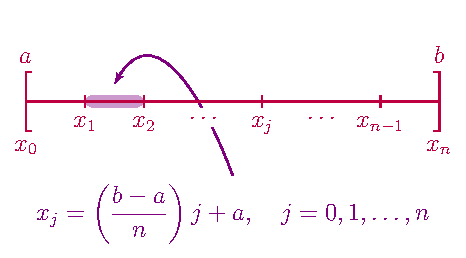
\includegraphics{Figuras/partição integral.pdf}
\end{figure}
%
Defina $\Delta x_j = x_{j+1} - x_j = (b-a)/n$ para cada $j = 0, 1, \dots, n-1$.
Defina também
%
\[
g_n(z) = \sum_{j=0}^{n-1} f(z, x_j)\Delta x_j = \frac{b-a}{n}\sum_{j=0}^{n-1} f(z, x_j).
\]
%
Observe que, por hipótese, cada uma das $f(z, x_j)$ é holomorfa. Suponha que 
$\overline{D(z_0,r)} \subseteq U$ para um $r$ suficientemente pequeno. Afirmamos que
$g_n\big|_{D(z_0, r)}$ converge uniformemente para $g\big|_{D(z_0, r)}$.
%
\begin{figure}[H]\centering
    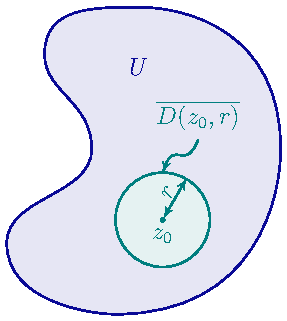
\includegraphics{Figuras/bola em U.pdf}
\end{figure}
%
De fato, por hipótese temos $f:U\times[a,b]\to\C$ contínua de modo que, pelo teorema anterior,
$f\big|_{\overline{D(z_0, r)} \times [a,b]}$ é uniformemente contínua. Portanto, dado $\e>0$
existe $\delta > 0$ tal que se $|x - y| < \delta$ então
%
\[
\sup_{z\in\overline{D(z_0,r)}} |f(z,x) - f(z,y)| < \frac{\e}{b-a}.
\]
%
seja
%
\[
M = \sup\left\{ |f(z,x)| : z\in\overline{D(z_0,r)}, x\in[a,b] \right\} < +\infty
\]
%
e tome $n\in\N$ tal que
%
\[
\frac{1}{n} < \min\left\{ \delta, \frac{\e}{M(b-a)} \right\}.
\]
%
\begin{figure}[H]\centering
    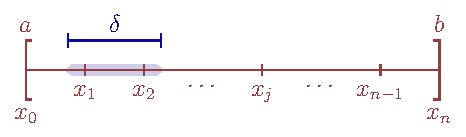
\includegraphics{Figuras/partição delta.pdf}
\end{figure}
%
Sendo assim, para todo $z\in D(z_0, r)$ vale
%
\begin{align*}
    |g_n(z) - g(z)| &= \left| \frac{b-a}{n}\sum_{j=0}^{n-1} f(z,x_j) 
                    - \int_a^b f(z,x) \, dx \right| \\[0.3cm]
                    &= \left| \frac{b-a}{n}\sum_{j=0}^{n-1} f(z,x_j) 
                    - \sum_{j=0}^{n-1}\int_{x_j}^{x_{j+1}} f(z,x) \, dx \right| \\[0.3cm]
                    &= \left| \sum_{j=0}^{n-1}\int_{x_j}^{x_{j+1}} f(z,x_j) \, dx
                    - \sum_{j=0}^{n-1}\int_{x_j}^{x_{j+1}} f(z,x) \, dx \right| \\[0.3cm]
                    &= \left| \sum_{j=0}^{n-1}\int_{x_j}^{x_{j+1}} f(z,x_j) - f(z,x) \, dx 
                    \right| \\[0.3cm]
                    &\leq \sum_{j=0}^{n-1}\int_{x_j}^{x_{j+1}} |f(z,x_j) - f(z,x)| \, dx \\[0.3cm]
                    &\leq \sum_{j=0}^{n-1} \frac{\e}{b-a}\cdot\frac{b-a}{n} \\[0.3cm]
                    &= \e,
\end{align*}
%
ou seja, $g_n\to g$ uniformemente em $D(z_0,r)$. Como $g_n$ é holomorfa para todo $n\in\N$
e a convergência é uniforme em $D(z_0,r)$, podemos garantir que $g$ é holomorfa em $D(z_0,r)$.
Daí, como $z_0$ é arbitrário, segue que $g$ é holomorfa em todo $U$.
\end{proof}
%
\begin{teorema}[Teorema de Fubini]
\label{teo-fubini-integrais-complexas}
\index{Teorema!de Fubini}
Seja $f:I\times U \subseteq \R\times\C \to\C$ uma função tal que
%
\begin{itemize}
    \item $f\big|_{[a,b]\times K}$ é limitada para todos $[a,b]\subseteq I$ e $K\subseteq U$
    compactos;
    \item $s\mapsto f(s, z_0)$ é uma função contínua por partes para cada $z_0\in U$ fixado;
    \item $s\mapsto f(s, z_0)$ e $s\mapsto f(s, z_1)$ são descontínuas nos mesmos pontos
    para todos $z_0, z_1\in U$;
    \item $z\mapsto f(s_0, z)$ é uma função contínua para cada $s_0\in I$ fixado.
\end{itemize}
%
Então, podemos afirmar que
%
\[
\int_{\y} \left( \int_a^b f(s,z) \, ds \right) \, dz 
= \int_a^b \left( \int_{\y} f(s,z) \, dz \right) \, ds,
\]
%
sendo $[a,b]\subseteq I$ e $\y\subseteq U$ um caminho suave por partes.
\end{teorema}
%
\begin{proof}
Seja $f(s, z) = u(s, z) + iv(s, z) = u(s, x, y) + iv(s, x, y)$, com $z = x+iy$. Temos que
%
\begin{align*}
    \int_{\y} \left( \int_a^b f(s,z) \, ds \right) \, dz 
    &= \int_{\y} \left( \int_a^b u(s,z) + iv(s,z) \, ds \right) \, dz \\
    &= \int_{\y} \left( \int_a^b u(s,z) \, ds + i\int_a^b v(s,z) \, ds \right) \, dz \\
    &= \int_0^1 \left( \int_a^b u(s,\y(t)) \, ds + i\int_a^b v(s,\y(t)) \, ds \right) \y'(t) \, dt \\
    &= \int_0^1 \left[ 
    \left( \int_a^b u(s,\y(t)) \, ds \right) x'(t) 
    - \left( \int_a^b v(s,\y(t)) \, ds \right) y'(t) 
    \right] \, dt \\
    &+
    i\int_0^1 \left[ 
    \left( \int_a^b u(s,\y(t)) \, ds \right) y'(t) 
    + \left( \int_a^b v(s,\y(t)) \, ds \right) x'(t) 
    \right] \, dt \\
    &= \int_0^1\int_a^b u(s,\y(t)) x'(t) \, ds \, dt 
    - \int_0^1\int_a^b v(s,\y(t)) y'(t) \, ds \, dt \\
    &+ i\left[
    \int_0^1\int_a^b u(s,\y(t)) y'(t) \, ds \, dt
    + \int_0^1\int_a^b v(s,\y(t)) x'(t) \, ds \, dt
    \right] \\
    &= \int_a^b\int_0^1 u(s,\y(t)) x'(t) \, ds \, dt 
    - \int_a^b\int_0^1 v(s,\y(t)) y'(t) \, ds \, dt \\
    &+ i\left[
    \int_a^b\int_0^1 u(s,\y(t)) y'(t) \, ds \, dt
    + \int_a^b\int_0^1 v(s,\y(t)) x'(t) \, ds \, dt
    \right] \\
    &= \int_a^b\left[
    \int_0^1 u(s,\y(t)) x'(t) \, dt - \int_0^1 v(s,\y(t)) y'(t) \, dt
    \right] \, ds \\
    &+ i\int_a^b\left[
    \int_0^1 u(s,\y(t)) y'(t) \, dt + \int_0^1 v(s,\y(t)) x'(t) \, dt
    \right] \, ds \\
    &= \int_a^b\left[
    \int_0^1 \left( u(s,\y(t)) x'(t) - v(s,\y(t)) y'(t) \right) \, dt 
    \right] \, ds \\
    &+ i\int_a^b\left[
    \int_0^1 u(s,\y(t)) y'(t) \, dt + \int_0^1 v(s,\y(t)) x'(t) \, dt
    \right] \, ds \\
    &= \int_a^b
    \int_0^1 \left( u(s,\y(t)) x'(t) - v(s,\y(t)) y'(t) \right) \, dt \\
    &+ i\left[
    \int_0^1 \left( u(s,\y(t)) y'(t) + u(s,\y(t)) x'(t) \right) \, dt
    \right] \, ds \\
    &= \int_a^b \Bigg[ \int_0^1 \big[
    \left( u(s,\y(t)) x'(t) - v(s,\y(t)) y'(t) \right) \\
    &+ i\left( u(s,\y(t)) y'(t) + v(s,\y(t)) x'(t) \right) \big] \, dt \Bigg] \, ds.
\end{align*}
%
Dessa última igualdade, concluímos finalmente que
%
\[
\int_{\y} \left( \int_a^b f(s,z) \, ds \right) \, dz 
= \int_a^b \left( \int_{\y} f(s,z) \, dz \right) \, ds.
\]
%
\end{proof}
%
\begin{corolario}
Se $f: I \times U \subseteq \R \times \C \to \C$ é uma função contínua, então
dados $-\infty < a < b < +\infty$ com $[a,b] \subseteq I$ e $\y\subseteq U$ um
caminho suave por partes, temos
%
\[
\int_{\y} \left( \int_a^b f(s,z) \, ds \right) \, dz 
= \int_a^b \left( \int_{\y} f(s,z) \, dz \right) \, ds.
\]
%
\end{corolario}
%
Apresentamos a seguir dois exemplos que nos serão úteis quando falarmos da
função gama e da função zeta de Riemann, respectivamente.
\begin{exemplo}
Sejam $0 < \delta < M < +\infty$ e
%
\[
S_{\delta, M} = \left\{ z\in\C : \delta < \Re(z) < M \right\}.
\]
%
Para cada $n\in\N$, considere $f:[1/n,n] \times S_{\delta, M} \to \C$ dada por
$f(s,t) = e^{-t} e^{(s-1)\ln t}$. Observe que $f$ é contínua, de modo que
podemos aplicar o teorema anterior para dizer que
$g_n:S_{\delta, M} \to \C$ dada por
%
\begin{align*}
    g_n(s) &= \int_{1/n}^n e^{-t}t^{s-1} \, dt \\
           &= \int_{1/n}^n e^{-t}e^{(s-1)\ln t} \, dt
\end{align*}
%
é holomorfa em $S_{\delta, M}$.
\end{exemplo}
%
\begin{exemplo}
Para cada $n\in\N$, considere $g_n:\{ \Re(s) > 0 \} \to \C$ dada por
%
\[
g_n(s) = \int_n^{n+1} \frac{x - \lfloor x \rfloor}{x^{s+1}} \, dx.
\]
%
Considere também a função auxiliar 
$f: [n, n+1]\times \{ \Re(s) > 0 \} \to \C$ 
dada por
%
\[
f(s,x) = \frac{x - \lfloor x \rfloor}{x^{s+1}}.
\]
%
Observe que esta função auxiliar não é uma função contínua.
%
\begin{figure}[H]\centering
    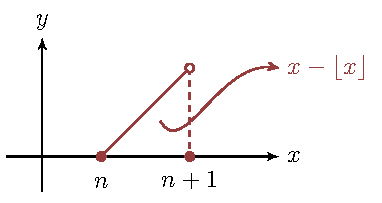
\includegraphics{Figuras/x - floor(x).pdf}
\end{figure}
%
De fato, para qualquer $s\in \{ \Re(s) > 0 \}$ fixado temos
%
\[
\lim_{x\to (n+1)^-} f(s,x)
%= \lim_{x\to (n+1)^-} \frac{x - \lfloor x \rfloor}{x^{s+1}}
= \frac{1}{(n+1)^{s+1}}
\neq 0 
= \frac{n+1 - \lfloor n+1 \rfloor}{(n+1)^{s+1}}
= f(s,n+1).
\]
%
Não obstante, note que
%
\begin{align*}
    |x^{s+1}| &= \left|\exp((s+1)\ln x)\right| \\
              &= \left|\exp\left( \Re(s) + 1 + i\Im(s) \right) \ln x\right| \\
              &= \exp\left( (\Re(s) + 1)\ln x \right) \\
              &\geq \exp\left( (\Re(s) + 1)\ln n \right) > 0, \, \forall x\in [n,n+1].
\end{align*}
%
Também temos, para todo $x\in[n,n+1]$, que $|x - \lfloor x \rfloor| \leq 1$. Portanto,
%
\[
|f(s,x)| \leq \frac{1}{\exp\left( (\Re(s) + 1)\ln n \right)}, \, 
\forall (s,x) \in \left\{ \Re(s) > 0 \right\}\times[n,n+1].
\]
%
Como as descontinuidades de $f$ ocorrem apenas nos pontos da forma $(s,n+1)$, podemos
usar o Teorema de Fubini para deduzir que, dado qualquer caminho triangular
$\Delta \subseteq \left\{ \Re(s) > 0 \right\}$, temos
%
\begin{align*}
    \int_{\Delta} g_n(s) \, ds 
    &= \int_{\Delta} \int_n^{n+1} \frac{x - \lfloor x \rfloor}{x^{s+1}} \, dx \, ds 
    \\[0.3cm]
    &= \int_n^{n+1} \int_{\Delta} \frac{x - \lfloor x \rfloor}{x^{s+1}} \, ds \, dx 
    \\[0.3cm]
    &= \int_n^{n+1} (x - \lfloor x \rfloor) 
    \left(\int_{\Delta} \frac{1}{x^{s+1}} \, ds \right) \, dx
    \\[0.3cm]
    &= \int_n^{n+1} (x - \lfloor x \rfloor) 
    \left(\int_{\Delta} e^{-(s+1)\ln x} \, ds \right) \, dx 
    \\[0.3cm]
    &= 0.
\end{align*}
%
Vamos verificar agora que o mapa $s\longmapsto g_n(s)$ define uma função contínua em 
$\left\{ \Re(s) > 0 \right\}$. 

De fato, para qualquer $s_0\in \left\{ \Re(s) > 0 \right\}$ fixado, temos:
\begin{align*}
    |g_n(s_0)-g_n(s)|
    &=
    \left|  
    \int_n^{n+1} \frac{x - \lfloor x \rfloor}{x^{s_0+1}} \, dx
    -
    \int_n^{n+1} \frac{x - \lfloor x \rfloor}{x^{s+1}} \, dx
    \right|
    \\[0.3cm]
    &=
    \left| 
        \int_n^{n+1} 
        \frac{x - \lfloor x \rfloor}{x^{s_0+1}} 
        - 
        \frac{x - \lfloor x \rfloor}{x^{s+1}}
        \, dx
    \right|
   \\[0.3cm]
    &= 
    \left| 
        \int_n^{n+1}
        \left(\frac{x - \lfloor x \rfloor}{x}\right)
        \left(\frac{1}{x^{s_0}} - \frac{1}{x^{s}}\right)
        \, dx
    \right|
   \\[0.3cm]
    &= 
    \left| 
        \int_n^{n+1}
        \left(\frac{x - \lfloor x \rfloor}{x}\right)
        \left(e^{-s_0\ln x} - e^{-s\ln x}\right)
        \, dx
    \right|
   \\[0.3cm]
    &\leqslant  
    \int_n^{n+1}
    \left|\frac{x - \lfloor x \rfloor}{x}\right|
    \left|e^{-s_0\ln x} - e^{-s\ln x}\right|
    \, dx
   \\[0.3cm]
    &\leqslant 
    \frac{1}{n}
    \int_n^{n+1}
    |e^{-s_0\ln x} - e^{-s\ln x}|
    \, dx
   \\[0.3cm]
    &\leqslant 
    \frac{1}{n}
    \int_n^{n+1}
    \left| \int_{s_0\ln x}^{s\ln x}e^{-z} \, dz\right|
    \, dx
   \\[0.3cm]
    &\leqslant 
    \frac{1}{n}
    \int_n^{n+1}
    \left[\int_{s_0\ln x}^{s\ln x}|e^{-z}| \, |dz|\right]
    \, dx
   \\[0.3cm]
    &\leqslant 
    \frac{1}{n}
    \int_n^{n+1}
    \left[
    e^{(|s|+|s_0|)\ln x}
    \cdot (\ln x)|s-s_0|
    \right]
    \, dx
   \\[0.3cm]
    &\leqslant 
    \left[
    e^{(|s|+|s_0|)\ln(n+1)}
    \ln(n+1)
    \right]
    |s-s_0|,
\end{align*}
Tomando limite, quando $s\to s_0$, em ambos lados da desigualdade acima verificamos que
\[
\lim_{s\to s_0}
|g_n(s_0)-g_n(s)|
\leqslant 
\lim_{s\to s_0}
\left[e^{(|s|+|s_0|)\ln(n+1)}\ln(n+1)\right]|s-s_0|
=
0.
\]
O que prova a afimarção que $g_n$ é uma função contínua em 
$\left\{ \Re(s) > 0 \right\}$. 
Usando este fato e lembrando que $\int_{\Delta} g_n(s) \, ds=0$,
para todo triângulo $\Delta$ contido em $\left\{ \Re(s) > 0 \right\}$,
temos garantidas todas as hipóteses do Teorema de Morera e assim podemos finalmente concluir que $g_n$ é holomorfa em $\left\{ \Re(s) > 0 \right\}$.



\bigskip 



Agora, note que para todos $n\in\N$ e $s\in\left\{ \Re(s) > 0 \right\}$ temos
%
\begin{align*}
    |g_n(s)| &= \left| \int_n^{n+1} \frac{x - \lfloor x \rfloor}{x^{s+1}} \, dx \right| \\
             &\leq \int_n^{n+1} \frac{1}{x^{\Re(s) + 1}} \, dx \\
             &= -\frac{x^{-\Re(s)}}{\Re(s)}\Bigg|_n^{n+1} \\
             &= \frac{1}{\Re(s)}\left( \frac{1}{n^{\Re(s)}} - \frac{1}{(n+1)^{\Re(s)}} \right).
\end{align*}
%
Sendo assim, temos para todo $k\in\N$
%
\begin{align*}
    \sum_{n=1}^k |g_n(s)| 
    &\leq \frac{1}{\Re(s)}\sum_{n=1}^k\left( \frac{1}{n^{\Re(s)}} - \frac{1}{(n+1)^{\Re(s)}} \right) \\
    &= \frac{1}{\Re(s)} 
    \left( 1 - \frac{1}{2^{\Re(s)}} 
    + \frac{1}{2^{\Re(s)}} - \frac{1}{3^{\Re(s)}} 
    + \cdots +
    \frac{1}{k^{\Re(s)}} - \frac{1}{(k+1)^{\Re(s)}} \right) \\
    &= \frac{1}{\Re(s)} \left( 1 - \frac{1}{(k+1)^{\Re(s)}} \right) 
    \xrightarrow{k\to\infty} \frac{1}{\Re(s)} < +\infty.
\end{align*}
%
Portanto,
%
\[
\sum_{n=1}^{\infty} |g_n(s)| \leq \frac{1}{\Re(s)}, \, 
\forall s\in\left\{ z\in\C : \Re(z) > 0 \right\}.
\]
%
Restringindo nossa análise para $s\in\left\{ z\in\C : \Re(z) > \delta \right\}$, $\delta > 0$,
obtemos a seguinte cota, que é uniforme em $s$
%
\[
\sum_{n=1}^{\infty} |g_n(s)| \leq \frac{1}{\delta}.
\]
%
Pelo Teste M de Weierstrass, segue que a sequência de funções
%
\[
S_k \equiv \sum_{n=1}^{k} |g_n(s)|
\]
%
converge uniformemente em $\left\{ z\in\C : \Re(z) > \delta \right\}$ para alguma função
holomorfa $S_b: \left\{ z\in\C : \Re(z) > \delta \right\} \to \C$.

Por outro lado, sabemos que a função $S$ dada por
%
\[
s \mapsto \sum_{n=1}^{\infty} g_n(s)
\]
%
está bem definida em $\left\{\Re(s) > 0 \right\}$. Como 
$S\big|_{\left\{ z\in\C : \Re(z) > \delta \right\}}$ é holomorfa, segue que $S$ é holomorfa em
$\left\{\Re(s) > 0 \right\}$. Equivalentemente,
%
\begin{align*}
    S(s) &= \sum_{n=1}^{\infty} g_n(s) \\
         &= \sum_{n=1}^{\infty} \int_n^{n+1} \frac{x - \lfloor x \rfloor}{x^{s+1}} \, dx \\
         &= \int_1^{\infty} \frac{x - \lfloor x \rfloor}{x^{s+1}} \, dx
\end{align*}
%
é holomorfa em $\left\{ z\in\C : \Re(z) > \delta \right\}$.
\end{exemplo}
%